% flashcards-title: Cross-product direction in the page plane
% flashcards-desc: From a common tail, vector A points right along positive x and vector B points up along positive y. A question mark asks whether the perpendicular result is out of or into the page.
\documentclass[border=5mm]{standalone}
\def\pgfsysdriver{pgfsys-dvisvgm.def}
\usepackage{tikz}
\usetikzlibrary{arrows.meta,calc,patterns.meta,positioning}
\renewcommand{\familydefault}{\sfdefault}

\definecolor{fcInk}{HTML}{1C1C1E}
\definecolor{fcMuted}{HTML}{68686D}
\definecolor{fcGuide}{HTML}{C9C9CE}
\definecolor{fcGold}{HTML}{D7A313}
\definecolor{fcGoldSoft}{HTML}{F8E8AE}

\tikzset{
  fc canvas/.style={fill=white, rounded corners=2.5mm},
  fc vector/.style={
    draw=fcGold,
    line width=1.35mm,
    line cap=round,
    -{Stealth[length=4.1mm,width=3.25mm]}
  },
  fc vector secondary/.style={
    draw=fcInk,
    line width=1.15mm,
    line cap=round,
    dash pattern=on 4.1mm off 2.6mm,
    -{Stealth[length=3.9mm,width=3.1mm]}
  },
  fc resultant/.style={
    draw=fcMuted,
    line width=1.55mm,
    line cap=round,
    -{Stealth[length=4.6mm,width=3.6mm]}
  },
  fc axis/.style={
    draw=fcInk,
    line width=.72mm,
    -{Stealth[length=3.1mm,width=2.5mm]}
  },
  fc guide/.style={
    draw=fcMuted,
    line width=.55mm,
    dash pattern=on 2.3mm off 1.8mm
  },
  fc construction/.style={draw=fcGuide, line width=.32mm},
  fc endpoint/.style={circle, fill=fcInk, inner sep=1.45mm},
  fc label/.style={font=\bfseries\large, text=fcInk},
  fc small label/.style={font=\small, text=fcMuted},
  fc caption/.style={font=\bfseries\small, text=fcMuted}
}

\begin{document}
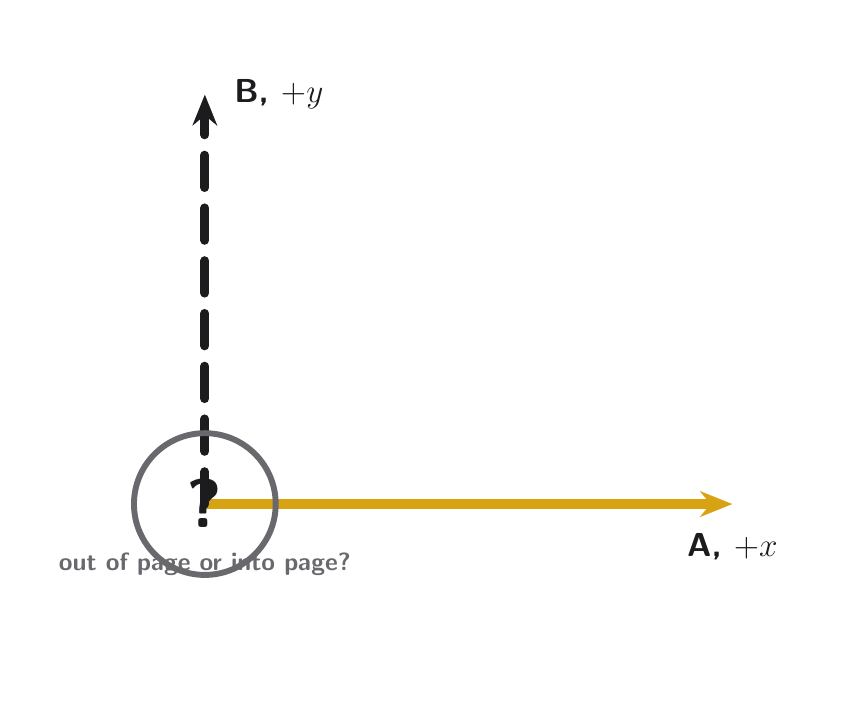
\begin{tikzpicture}[x=1cm,y=1cm]
  \path[fc canvas] (-1.1,-1.1) rectangle (8.9,7.2);
  \coordinate (O) at (1.15,1.15);
  \coordinate (A) at (7.85,1.15);
  \coordinate (B) at (1.15,6.35);

  \draw[fc vector] (O) -- (A);
  \draw[fc vector secondary] (O) -- (B);
  \node[fc label, below=2.5mm] at (A) {A, $+x$};
  \node[fc label, right=2.5mm] at (B) {B, $+y$};

  \node[circle, draw=fcMuted, line width=.75mm, minimum size=18mm, font=\bfseries\Huge, text=fcInk] at (O) {?};
  \node[fc caption, below=5mm] at (O) {out of page or into page?};
\end{tikzpicture}
\end{document}
